%
% File:     example.tex
%
% Document based on the template for thesis and dissertations
% developed by Steven White and Malcolm Hutson.
%
% Extensively modified by Adam Lewis (awlewis@cacs.louisiana.edu) to
% meet the UL Graduate School requirements as of Spring 2011. 
%
% Unless otherwise expressly stated, this work is licensed under the
% Creative Commons Attribution-Noncommercial 3.0 United States License. To
% view a copy of this license, visit
% http://creativecommons.org/licenses/by-nc/3.0/us/ or send a letter to
% Creative Commons, 171 Second Street, Suite 300, San Francisco,
% California, 94105, USA.
%
% THE SOFTWARE IS PROVIDED "AS IS", WITHOUT WARRANTY OF ANY KIND, EXPRESS
% OR IMPLIED, INCLUDING BUT NOT LIMITED TO THE WARRANTIES OF
% MERCHANTABILITY, FITNESS FOR A PARTICULAR PURPOSE AND NONINFRINGEMENT.
% IN NO EVENT SHALL THE AUTHORS OR COPYRIGHT HOLDERS BE LIABLE FOR ANY
% CLAIM, DAMAGES OR OTHER LIABILITY, WHETHER IN AN ACTION OF CONTRACT,
% TORT OR OTHERWISE, ARISING FROM, OUT OF OR IN CONNECTION WITH THE
% SOFTWARE OR THE USE OR OTHER DEALINGS IN THE SOFTWARE.

\documentclass[12pt]{report}	% The documentclass must be ``report''.

% Dissertation package style file.
\usepackage{template/uldiss}  		

% 
% Here is a collection of optional packages that can make your life
% far more pleasant while writing your thesis, prospectus, or
% dissertation.   You should tailor these to match the specific needs
% for your document.
%
\usepackage{amsmath,amsthm,amsfonts,amscd,amssymb} % Some packages to write mathematics.
\usepackage{eucal} % Euler fonts
\usepackage{verbatim} % Allows quoting source with commands.
% The listings package supports the pretty-printing of source code.
% The listings packages supports the most commonly used programming
% languages.
\usepackage{listings}
\lstloadlanguages{Matlab,C++,C,Pascal}
\lstset{
         basicstyle=\footnotesize\ttfamily, 
         %numbers=left,              
         numberstyle=\tiny,          
         %stepnumber=2,              
         numbersep=5pt,              
         tabsize=2,                  
         extendedchars=true,         
         breaklines=true,            
         keywordstyle=textbf,    
         stringstyle=\ttfamily, 
         showspaces=false,       
         showtabs=false,         
         xleftmargin=17pt,
         framexleftmargin=17pt,
         framexrightmargin=5pt,
         framexbottommargin=4pt,
         %backgroundcolor=\color{lightgray},
         showstringspaces=false  
 }
% The caption package is used for fancy formatting of figure, table, and
% other captions.  It is very useful when combined with the listings package.
\usepackage{caption}
\DeclareCaptionFont{white}{\color{white}}
\DeclareCaptionFormat{listing}{\colorbox[cmyk]{0.43, 0.35, 0.35,0.01}{\parbox{\textwidth}{\hspace{15pt}#1#2#3}}}
\captionsetup[lstlisting]{format=listing,labelfont=white,textfont=white, singlelinecheck=false, margin=0pt, font={bf,footnotesize}}
\usepackage{pdfpages}
%
% The graphicx package is the standard package for importing of graphics
% into LaTeX documents.   Note that we configure the package to, by
% default, look for PNG, JPEG, and PDF files in a sub-directory of the
% current directory.
\usepackage{graphicx}
\DeclareGraphicsExtensions{.png,.jpg,.pdf}
\graphicspath{{graphics/}}
%
% Use the subfig package for dealing with multiple part figures.
\usepackage[caption=false,labelfont=sf,textfont=sf,captionskip=5pt]{subfig}
% 
% The comment package is useful when you use EMACS for editing LaTeX
% documents.  The table editor in EMACS orgtbl-mode interfaces with this
% package for easy editing of tables using the org-mode table editing
% functions. 
\usepackage{comment}

%% imported packages
%%
\usepackage{xargs}

\usepackage{mathpartir}
\usepackage{mathtools}
\usepackage{lambda,cc}
\usepackage[noshare]{vlc}
\usepackage{hyperref}
\usepackage{xcolor}
\usepackage{calc}
%\usepackage[labelformat=simple]{subcaption}
%\renewcommand\thesubfigure{(\alph{subfigure})}

\usepackage{stmaryrd}
\setcounter{tocdepth}{3}
\usepackage{makecell}
%\usepackage{setspace}

\usepackage[inline]{enumitem}
\usepackage{epstopdf}
\usepackage{booktabs}

\newcommand{\pg}{\ensuremath{p}}
\newcommand{\pgi}{\ensuremath{\pg_i}}
\newcommand{\pgj}{\ensuremath{\pg_j}}
\newcommand{\pgk}{\ensuremath{\pg_k}}

\newcommand{\seqijk}{\ensuremath{\dots,\pgi,\dots,\pgj,\dots,\pgk,\dots}}
\newcommand{\seqij}{\ensuremath{\dots,\pgi,\dots,\pgj,\dots}}


\newcommand{\sseqijk}{\ensuremath{\pg_1,\dots,\pgi,\dots,\pgj,\dots,\pgk,\dots}}

\newcommand{\pe}{\ensuremath{E}}

\newcommand{\pga}{\ensuremath{p_1}}
\newcommand{\pgb}{\ensuremath{p_3}}
\newcommand{\pgc}{\ensuremath{p_6}}

\newcommand{\nlevs}{\ensuremath{n}}
\newcommand{\tc}[1]{\ensuremath{O(#1)}}

\newcommand{\ongoing}{{}}
\newcommand{\temp}[1]{\textcolor{green}{\textbf{#1}}}

\newcommand{\toolS}{SHErrLoc}
\newcommand{\toolM}{\textsc{Mycroft}}
\newcommand{\toolD}{DOMSTED}
\newcommand{\toolMin}{MinErrLoc}
\newcommand{\toolH}{Helium}
\newcommand{\toolSk}{Skalpel}
\newcommand{\toolCh}{Chameleon}
\newcommand{\toolCf}{CFT}

\newcommand{\cs}{\ensuremath{\mathcal S}}
\newcommand{\con}{\ensuremath{C}}

\newcommand{\tv}{\ensuremath{\alpha}}
\newcommand{\tvf}{\ensuremath{\alpha_1}}
\newcommand{\tvs}{\ensuremath{\alpha_2}}
\newcommand{\tvt}{\ensuremath{\alpha_3}}
\newcommand{\tvv}{\ensuremath{\beta}}
\newcommand{\tvvf}{\ensuremath{\beta_1}}

\newcommand{\cname}{category}
\newcommand{\cnames}{categories}
\newcommand{\Cname}{Category}


\newcommand{\typel}{\prog{location}}
\newcommand{\typet}{\prog{type}}
\newcommand{\typer}{\prog{reason}}
\newcommand{\typee}{\prog{expression}}
\newcommand{\typeT}{\prog{Type}}
\newcommand{\typeR}{\prog{Reason}}
\newcommand{\typeE}{\prog{Expression}}
\newcommand{\typeL}{\prog{Location}}

\newcommand{\std}{\textit{std}}

\newcommand{\progsq}[1]{\prog{\textquotesingle#1\textquotesingle}}
\newcommand{\progdq}[1]{\prog{"#1"}}
\newcommand{\subele}[2]{$#1_{#2}$}
\newcommand{\arr}{$\to$}
%\newcommmand{\arrtp}[2]{$#1 \to #2$}
\newcommand{\newCompiler}{\textsc{Learnskell}}
\newcommand{\lines}[2]{Lines (#1-#2) omitted for brevity}
\newcommand{\TypeDiff}{\textit{TypeDiff}}
\newcommand{\TopDiff}{\textit{TopDiff}}
\newcommand{\BDiff}{\textit{BDiff}}
\newcommand{\TopLevelDiff}{\textit{TopFuncDiff}}
\newcommand{\TopBracketDiff}{\textit{TopBracDiff}}
\newcommand{\FuncDiff}{\textit{FuncDiff}}
\newcommand{\BracketDiff}{\textit{BracDiff}}
\newcommand{\TypeDiffs}{\textit{TypeDiffs}}
\newcommand{\TopDiffs}{\textit{TopDiffs}}
\newcommand{\BDiffs}{\textit{BDiffs}}
\newcommand{\TopLevelDiffs}{\textit{\TopLevelDiff{s}}}
\newcommand{\FuncDiffs}{\textit{FuncDiffs}}
\newcommand{\BracketDiffs}{\textit{\BracketDiff{s}}}
\newcommand{\Unify}{\textit{Unify}}
\newcommand{\where}{\textit{where}}
\newcommand{\otherwise}{\textit{otherwise}}
\newcommand{\Similarity}{\textit{Similarity}}
\newcommand{\smallwedge}{\mathrel{\text{\raisebox{0.25ex}{\scalebox{0.8}{$\wedge$}}}}}
\newcommand{\smallvee}{\mathrel{\text{\raisebox{0.25ex}{\scalebox{0.8}{$\vee$}}}}}
\newcommand{\tempPercent}[1]{\textbf{\textcolor{red}{#1\%}}}
\newcommand{\Ifit}{\textit{If}}
\newcommand{\ifit}{\textit{if}}
\newcommand{\thenit}{\textit{then}}
\newcommand{\andit}{\textit{and}}
\newcommand{\is}{\textit{is}}
\newcommand{\form}{\textit{form}}
\newcommand{\FE}{\textit{FE}}
\newcommand{\data}{\mathcal{D}}
\newcommand{\Var}{\textit{Var}}
\newcommand{\M}{\mathcal{M}}
\newcommand{\E}{\mathcal{E}}
\newcommand{\X}{\mathcal{X}}
\newcommand{\N}{\mathcal{N}}
\newcommand{\tp}{t_p}
\newcommand{\tn}{t_n}
\newcommand{\fp}{f_p}
\newcommand{\fn}{f_n}
\newcommand{\pr}{\textit{pr}}
\newcommand{\re}{\textit{re}}

\renewcommand{\progind}{0pt}
\newcommand{\cL}{{\cal L}}
\newcommand{\parag}[1]{\medskip\noindent\textbf{#1}\ \ }
\newcommand{\smote}{SMOTE}
\newcommand{\studySubmission}{226}
\newcommand{\randomForest}{Random-Forest}
\newcommand{\benchf}{Haskell-1}
\newcommand{\benchs}{Haskell-2}
\newcommand{\bencht}{Haskell-3}
\newcommand{\benchl}{Haskell-3}
\newcommand{\years}{\benchf}
\newcommand{\yeart}{\benchs}
%
\newcommand{\pui}[2]{\ensuremath{\prog{#1} =^? \prog{#2}}}
%
\newcommand{\mui}[2]{\ensuremath{#1 =^? #2}}

\newcommand{\mt}{\ensuremath{\tau}}

\newcommand{\mtexp}{\ensuremath{\mt_{\textit{exp}}}}
\newcommand{\mtinf}{\ensuremath{\mt_{\textit{inf}}}}


\newcommand{\ualg}{\ensuremath{\mathcal U}}
\newcommand{\dalg}{\ensuremath{\mathcal D}}
\newcommand{\td}{\textit{TD}}
\newcommand{\subtt}{\ensuremath{\theta}}
\newcommand{\sieves}{\textit{TD}}

\newcommand{\nameva}{(a)}
\newcommand{\namevb}{(b)}
\newcommand{\namevc}{(c)}
\newcommand{\namevd}{(d)}
\newcommand{\nameve}{(e)}
\newcommand{\namevf}{(f)}
\newcommand{\namevg}{(g)}
\newcommand{\namevh}{(h)}
\newcommand{\namevi}{(i)}
\newcommand{\namevj}{(j)}
\newcommand{\namevk}{(k)}
\newcommand{\namevl}{(l)}

\newcommand{\level}{\textit{lev}}
\newcommand{\union}[2]{\ensuremath{#1 \cup #2}}
\newcommand{\idx}{\textit{idx}}
\newcommand{\depth}{\textit{depth}}
\newcommand{\length}{\textit{numArity}}

\newcommand{\mtf}{\ensuremath{\mt_1}}
\newcommand{\mts}{\ensuremath{\mt_2}}

\newcommand{\restrict}[2]{\ensuremath{#1|_{#2}}}

\newcommand{\nextIdx}[2]{\ensuremath{\textit{next}(#1,#2)}}

\newcolumntype{Y}{>{\centering\arraybackslash}X}

\newcommand{\intVal}{integral}
\newcommand{\IntVal}{Integral}

\newtheorem{theorem}{Theorem}
\newtheorem{definition}{Definition}

\newcommand{\trainset}{Year-03}
\newcommand{\evalset}{Year-02}

\newcommand{\location}{Location}
\newcommand{\reason}{Reason}
\newcommand{\correct}{Specific}
\newcommand{\concrete}{Concrete}
\newcommand{\Location}{Location}
\newcommand{\Reason}{Reason}
\newcommand{\Correct}{Specific}
\newcommand{\Concrete}{Concrete}
\newcommand{\newTool}{\textsc{MLPEx}}
















%\sloppy
%\sloppypar

\renewcommand{\progind}{0pt}
\newcommand{\cL}{{\cal L}}
\newcommand{\parag}[1]{\medskip\noindent\textbf{#1}\ \ }
\newcommand{\newCompiler}{\textsc{Learnskell}}
%% end importing
%%

%\usepackage{draftwatermark}	% Uncomment this line to have the
				% word, "DRAFT," as a background
				% "watermark" on all of the pages of
				% of your draft versions. When ready
				% to generate your final copy, re-comment
				% it out with a percent sign to remove
				% the word draft before you run
				% latex for the last time.
%
% Document Type
%
% Choose a document type by commenting out every other type.
%\prospectus
\dissertation
%\masterthesis
%\masterreport


%
% School Customizations 
%
% Select your school
% If your school is not listed, this template has not been specifically  
%   customized for you yet, but the Grad School requirements will be met.
%   Try one that might be similar.

\cacscmps
%   ACM Transactions bibliography

%\cacseecs
%   ACM Transactions bilbiography

%\schoolofmusic
%   Chicago style bibliography with footnotes?

%
% Basic Information
%

\author{Baijun Wu}
% Your name how it should normally appear across the document.
% The graduate school requires that your name always appear identically
%   every time that it is used. To help, we recommend use \theauthor
%   wherever your name should be printed for consistency.

\properauthor{Baijun Wu}
% Your proper name for alphabetizing. (Used in the abstract.)
% Last, First Middle Suffix

\title{Towards To User Friendly Error Debugging}
% The title of your thesis/dissertation. Use a tilde (~) for any
%   spaces that should not be broken at line breaks.

\dean{C. E. Palmer}
 % The Dean of the Graduate School

%\degree{Master of Science}
% The full title of your degree. 
% The default value is guessed by the document type and school.
  
%\major{Computer Science}
  % Your major.
  % The default value is guessed by your school.

%\graduationmonth{Spring}      
% Graduation semester, either Spring, Summer, or Fall, in the form
% as `\graduationmonth{Fall}'. Do not abbreviate.
% The default value (either Spring, Summer, or Fall) is guessed
% according to the time of running LaTeX.

% \graduationyear{2010} Graduation year, in the form as
% `\graduationyear{2001}'.  Use a 4 digit (not a 2 digit)
% number.  The default value is guessed according
%to the time of running LaTeX.
  
\previousdegrees{
Bachelor of Science, Sichuan University, 2008; 
Master of Science, Sichuan University, 2011; 
Doctor of Philosophy, University of Louisiana at Lafayette, \thegraduationmonth \ \thegraduationyear
}
% List all of your degrees, including the degree you are seeking with
% this document!

\abstractwordcount{120}
% The number of words in your abstract.
 % Unfortunately there is no clean way to count words in a section in Latex.
  
%
%
% Enter names of the member(s) of your committee. 
% Put one name per line with the name in square brackets. 
% The name on the last line, however, must be in curly braces.
%
% NOTE: The first member should be your supervisor.
%
% NOTE: Maximum six members. Minimum one member (supervisor).
%
\committeemembers
	[Erwin Schr\"odinger]
	{Albert Einstein}
	
\committeememberstitle
	[Professor of Physics]
	{Adjunct Professor of Math}

%\supervisortitle{Dr.}   
  % Your supervisor's title (Dr., Mrs., Mr., Sir, etc)
  %
  % The default value is "Dr."

%
% Change the	Hyphenation behavior.
%
%
\hyphenation{FORTRAN Hy-phen-a-tion}
% Manually specify how certain words should be hyphenated, if needed.
% You may add words without hyphens to request that they not be hyphenated.

%\hyphenpenalty=100000
% If you want no hyphenation in your document at all, uncomment
%   this line to set the hyphen penalty to an unreasonably
%   high value. 

%
% Some optional commands to change the document's defaults.
%
%
%\singlespacing
%\oneandonehalfspacing

%\singlespacequote
%\oneandonehalfspacequote

%\topmargin 0.125in	% Adjust this value if the PostScript file output
			% of your dissertation has incorrect top and 
			% bottom margins. Print a copy of at least one
			% full page of your dissertation (not the first
			% page of a chapter) and measure the top and
			% bottom margins with a ruler. You must have
			% a top margin of 1.5" and a bottom margin of
			% at least 1.25". The page numbers must be at
			% least 1.00" from the bottom of the page.
			% If the margins are not correct, adjust this
			% value accordingly and re-compile and print again.
			%
			% The default value is 0.125" 

	
%
%The document starts here.
%

\makeindex              % Make the index

\begin{document}

\titlepage              % Produces the title page.

\copyrightpage          % Produces the copyright page.

\approvalpage           % Produces the approval page

%
% Dedication, epigraph, and/or acknowledgments are optional, but must
% occur here.
%
%
\begin{dedication}
Dedicated to the people who I really care about.
\end{dedication}

\begin{acknowledgments}		% Optional
Thank everyone....
\end{acknowledgments}

% Table of Contents will be automatically generated and placed here.
\tableofcontents   
% List of Tables will be placed here, if applicabl.e
\listoftables      
% List of Figures will be placed here, if applicabl.e
\listoffigures     

%
% Actual text starts here.%
%
% Including external files for each chapter makes this document simpler,
% makes each chapter simpler, and allows for generating test documents
% with as few as zero chapters (by commenting out the include statements).
% You can even change the chapter order by merely interchanging the order
% of the include statements.
%
%\include{chapter-introduction}

\chapter{Introduction}

In this dissertation, I present my research on type error debugging.
Understanding type error messages and fixing type errors is challenging for both novice and professional programmers.
Type errors can be caused for various reasons, for example, 
using wrong library functions,
using constants as functions, 
applying functions to arguments of wrong types, 
missing and having extra pairs of parentheses, and so on. 
In the first part of this dissertation, I present the insights about the type error debugging behaviors in practice, 
which are exploited to develop an effective error debugger in the later part of this dissertation.

This chapter motivates the needs of user friendly error messages
by investigating the challenges of debugging type errors.
It also outlines the structure of this dissertation and presents the contributions of this work.


\section{Motivation}
Type inference allows programs to be statically typed without
the presence of full type annotations. Most functional languages,
such as Haskell, ML, and OCaml support type inference, and many
imperative languages, such as C++, C\#, and Java, have started to
incorporate a limited form of type inference.
While type inference helps to save type annotations, learning languages
using type inference is quite challenging,
in particular for those who have background in imperative languages~\cite{clack1995dys,joosten1993teaching}.
Studies show that novice programmers tend to make type errors more often~\cite{chambers2012function,Heeren05:TQT,hage2006mining,tirronen2015understanding}, and
one reason may be that they have difficulties in learning modern type systems~\cite{clack1995dys,chakravarty2004risks}.


Understanding and fixing type errors is even harder~\cite{marceau2011measuring,marceau2011mind,tirronen2015understanding},
since type error messages generated by existing type checkers are usually ineffective~\cite{marceau2011mind}.
In particular, they may point to locations that are distant to real error causes,
expose errors in internal jargon, or provide misleading fixing suggestions.
Therefore, providing good quality type error messages
is important for beginners to study functional programming.

The problem of improving the quality of error messages has received
extensive attention. Many different approaches have been developed,
including error locating~\cite{Mcadam98:UST,Eo04:PSH,Zhang15:DTE,Pavlinovic14:FMT},
type error slicing for locating all the possible locations that
contribute to type errors~\cite{Schilling12:CFT,Haack03:TES},
inconsistency identification for finding program locations leading to
type conflicts~\cite{Yang00:ETE,Wazny06:TIT},
error explanation explaining why type errors occur and why certain
types are inferred~\cite{Chitil01:CET,jun2002explaining,Loncaric16:PFT},
error reparation that generates informative messages to fix type errors,
and interactive error debugging that allows users to move around
program ASTs and inspect the type of each node~\cite{Brassel04:TH,Chitil01:CET}.


While various methods have been proposed to locate
error causes more accurately and 
generate more informative change suggestions,
%improve the quality of error messages,
most of them work well under certain conditions.
Some methods~\cite{CE14popl,CE14flops,Zhang14:tgd}
work well when real error causes are
at leaves of ASTs. Others~\cite{Lerner06:SSM,Pavlinovic15:PST}
work well when there is only one type error but
not so well when there are multiple type errors.

%Therefore, we manually compute these statistical results and analyze them in our study.


\section{Research Goals}

So far, a good understanding about how type error debugging looks like
in practice is missing. As a result, it's unclear whether the conditions
for error debuggers to work well hold in practice or not.
%
There have been some efforts to collect relevant
information about errors made by students
~\cite{Hage09:Neon,tirronen2015understanding,chambers2012function,fenwick2009another,denny2012all}.
Neon~\cite{Hage09:Neon} is a domain specific language designed to query
program databases, which collected programs written by students learning Haskell.
It can extract various characteristics of the student programs,
for example, how the lengths of compiled modules evolve,
and how the average and median values of compilation intervals
change over a certain time period.
However, some information, like how far away is 
the error location
given by the type debugger from the real error cause,
can not be automatically generated by Neon.

A comprehensive overview of the mistakes made by beginners in Haskell was presented by \cite{tirronen2015understanding}.
The authors classified the errors made by students into three
categories: syntax errors, type errors, and run-time errors,
and then performed a fine-grained analysis for each category.
They showed some difficulties, like misuses of pattern matching,
in learning functional programming.
They also suggested that a more effective strategy of teaching type systems
is desirable.


While Neon and the overview study give some insights about kinds of errors the beginners of
functional programming made, they do not tell how errors were fixed and what students did.
%
This dissertation aims to address this problem by inspecting more than 2,700
ill-typed programs from 3 data sets,
recording various kinds of information about each type error, 
and analyzing the statistical results to extract high-level insights.
%
The empirical study results show that the type errors, arising from errors in grouping constructs like parentheses and brackets,
usually take more than 10 steps to fix and occur quite frequently in practice.
This class of errors is called as nontructural errors,
and existing error debuggers fail to generate precise and informative error messages for such errors.
In this dissertation, I will present a solution that delivers high quality error messages to fix nonstructural errors.


\section{Contributions and Outline of This Dissertation}

In this section, I present the structure of the remainder of this dissertation,
and along the way the contributions of this work are given.

Chapter~\ref{sec:review} (\emph{Literature Review}) collects research related to error debugging behaviors,  
type error debuggers and machine learning on programming languages.
This chapter contains material from \cite{wu2017type} and \cite{wu2017learning}.

Chapter~\ref{sec:background} (\emph{Background}) systematically explains under what conditions existing error debuggers work well
based on general ideas underlying many debuggers.
The result in this chapter is applicable to future debuggers that share the similar underlying ideas.
This chapter contains material from \cite{wu2017type}.

Chapter~\ref{sec:subjects} (\emph{Study Subjects}) presents the study subjects used in this work and
discuss the methodology used to study the process of fixing type errors based on the study subjects.
Five meaningful metrics are proposed to represent the real error debugging.
This chapter contains material from \cite{wu2017type}.

Chapter~\ref{sec:analysis} (\emph{Debugging Behavior Analysis}) shows the statistical results by analyzing the study subjects.
Many interesting observations that inform future research directions are derived.
This chapter contains material from \cite{wu2017type} and makes the following contributions.

\begin{enumerate}
\item The results in Section~\ref{sec:causes} show that about 45\% to 60\% of type errors are fixed by changing the structure of program ASTs 
and only about 22\% to 37\% of them are fixed by changing single leaves.
This indicates that most error debuggers won't work well in practice.

\item The results in Section~\ref{sec:annotation} show that on average about 30\% of type errors are caused by wrong type annotations.
This indicates that type annotations are unreliable for debugging ill-typed programs

\item The results in Section~\ref{sec:effectiveness} show that more concrete and precise error messages tend to be more effective for users to debug type errors.

\item The language features that cause type errors to be difficult to debug are presented in Section~\ref{sec:difficulty}.
The results indicate that function composition related operations (\prog{(.)}, \prog{\$} and parentheses),
point-free style function definitions, wrong type annotations, and wrong pattern matching often lead type error debugging to be challenging.
\end{enumerate}

Chapter~\ref{sec:features} (\emph{Nonstructural Type Error Representation}) presents the information extracted from error messages and program ASTs 
to represent nonstructural errors which are common in practice as shown in Chapter~\ref{sec:analysis}, but yet are handled poorly by existing debuggers.
Three kinds of information are considered: (1) the type conflicts, (2) the program structure around the error location,
and (3) the error messages from the underlying debugger.
This chapter contains material from \cite{wu2017learning} and makes the following contributions.

\begin{enumerate}
\item An algorithm for computing the differences between two types when they fail to unify is developed.
As error debuggers always use, among others, the heuristic of type difference of conflicting types to rank multiple error locations~\cite{Chen14:CFT,Hage07:HTE},
the proposed algorithm could be employed to develop more powerful error ranking heuristics.

\item In total 14 features are extracted to effectively represent nonstructural errors.
They provide a principled way to correlate type errors with program structures by covering a wide array of useful error information.
\end{enumerate}

Chapter~\ref{sec:solution} (\emph{Learning Nonstructural Errors}) provides the proposed debugger \newCompiler\ 
to generating user friendly error messages for nonstructural errors.
This capter contains material from \cite{wu2017learning} and makes the following contributions.

\begin{enumerate}
\item The motivation for using machine learning in developing an effective debugger for nonstructural errors is justified.

\item An algorithm for imbalanced classification problem is proposed to help determine if a type error is structural or nonstructural.

\item The evaluation results of the proposed solution are given, demonstrating that the machine learning-based error debugger is effective and scalable.
\end{enumerate}

Chapter~\ref{sec:conclusion} (\emph{Conclusion}) closes this dissertation with a summary of other applications of using machine learning in programming area,
the most important contributions of this work, and directions for future research.

\chapter{Literature Review}
\label{sec:review}

The work of type error debugging is related to various research areas, including
error understanding, debugging behaviors, the quality of error message,
and error debugger design.
This chapter collects the work related to all the study activities.

\section{Error Debugging Behaviors}
\label{sec:review:behavior}

This section provides the discussion about previous work that try to understand how students behave when learning programming languages.

\subsection{Comprehension of errors}

Student programs were collected and errors made by students
were analyzed by \cite{tirronen2015understanding}.
The authors investigated various compile-time and run-time errors
and presented the causes for different kinds of errors.
Their results showed that type errors prevalence in beginners' programs.
However, their work didn't try to understand how type
errors were fixed and what students did.
%Our work complements their findings on type error category with
%detailed information about how type error debugging of novice programmers looks like.

\cite{tirronen2014study} studied
errors that occurred in student programs and
provided a comprehensive description of
common difficulties in learning modern type systems.
However, the result is not from a statistical view.
This work presents similar findings in Section~\ref{xxx}
and explains the
reasons of difficulties from the view of error debugging.

\cite{hage2006mining} showed statistical
results of errors by mining the program database we used
in this paper.
Their result was extracted using the DSL Neon~\cite{Hage09:Neon}.
As the analysis was done automatically, the information that
could be obtained was limited. For example, it is impossible
to choose reference programs correctly, as we have shown that
the first type correct program after the ill-typed one is not
necessarily the reference program. It is also impossible to
extract all the information presented in this paper as
reference programs are needed to do so.

\subsection{Programmer response to errors}

\cite{chambers2012function} studied information sources programmers
usually refer to when debugging functional
programs.
Their observations showed that students used
code examples frequently
when encountered errors.
Their results support our finding in this paper that
student programs may diverge to the references
during error fixing process. Their study
considered only a few human subjects, while this study is
large scale and gives statical results.

\cite{munson2016analyzing}
showed that, when there are multiple errors,
the students who handle only the first error
instead of debugging all errors at once usually
performed better.
The authors showed positive correlation
between high assignment scores and
high probability of addressing only
the first error in presence of multiple errors.
%
They suggested that a good practice to fix
errors is to debug one error at a time.
In our analysis, we also observed that
students tended to handle one type error at each step.
This would be useful for novice programmers, especially
because there is a risk of producing bogus error messages
when multiple errors are present in
the same expression~\cite{Heeren05:TQT}.

\cite{marceau2011mind} investigated the interaction between
beginners and error messages.
The authors concluded that error messages were
inaccurate and not informative to students.
Their work proposed several design
suggestions for constructing IDEs and generating
error messages.
In contrast, this work gives insights
why error messages are ineffective.

\subsection{Effectiveness of error messages}

\cite{marceau2011measuring} proposed a set of metrics to
measure the effectiveness of
error messages.
They analyzed student edits
in response to error messages generated by DrRacket.
This work proposes a similar method to study
the relationship between
the concreteness of error messages and
error situations at a finer-grained level.

\cite{yang2000improved} defined a manifesto to show
what good error messages look like and discussed
the strengths and weakness of several type inference
algorithms based on it.
However, they did not provide justification
for their suggestions.
The results in this work support some of their claims,
like error messages
should be intuitive and source-based.

\cite{chen2014let} investigated the idea
of combining different error debuggers to improve
error locating precision. They also considered
an evaluation with the program database used
in this paper. While their work
chose the first programs that are well typed after
ill-typed programs as references, this work chooses
reference programs more appropriately by taking the
intentions of students into consideration.

\section{Type Error Debuggers}
\label{sec:reivew:debugger}

In this section, I discuss the relation between the solution proposed in this work to handle nonstructural errors and
three other lines of work: approaches that handle nonstructural errors, approaches that don't handle nonstructural errors,
and other applications of machine learning to solve programming language problems.

\subsection{Approaches that Handle Nonstructural Errors}

Helium \cite{Hage07:HTE} is a compiler that operates
on a graph representation of the constraints it generates
during type inference
and uses heuristics to present the most likely error cause. One
of these heuristics is the edit distance, which permutes leaves in
an AST to reorder function arguments or parts of a
tuple. It also tries to remove arguments or insert arguments and
then decides whether the resulting program would type check \cite{Heeren03:HLH}.
These heuristics work well in some cases. However, in many situations it
reports that functions have too few or too many arguments erroneously.
%as we saw earlier in the \prog{groepeer} example.
%and evaluation result in Section~\ref{sec:eval} The evaluation result doesn't mentions too few arguments, etc.
%
The problem is that the constraint
set generated is invalid, and these heuristics can't detect
the actual error cause and make a suggestion that will fix it.
%
The debugger \newCompiler\ proposed in this work doesn't suffer from this problem by learning
a relation between error situations (including conflicting types
and program structure around the error causes) and the correct fixes.


Seminal works by taking in an AST for the ill-typed program
and then proceeding to run a searcher over the AST and
making modifications that can remove nodes, change curried functions
to tupled functions and vice versa, change a 1-element list containing an n-tuple to an n-element list, or commute leaf nodes \cite{Lerner07:STM}.
In presence of multiple errors, it can apply triaging~\cite{Lerner07:STM}
to try and fix multiple type errors in different locations
It then employs heuristics to rank
these fixes. For example, it favors constructive changes over removals.
The modifications Seminal applies help to diagnose type
errors in many cases. However, Seminal suffers from
some problems. First, it doesn't work well when multiple errors
happen together because it's hard for Seminal to identify the error
cause, despite its triaging method.
%
Its approach to handling
multiple related errors is to systematically focus on a particular
expression and then remove sibling expressions until the type
error is removed. Once the first removal combination is found, it
proceeds to consider this case.
This prevents exponential explosions in complexity
that might come with considering all removal combinations,
but can often miss other error fixes. For the  \prog{groepeer}
example, it misses the error fix over \prog{drop n x}.
%
Second, Seminal doesn't scale well to large programs.
For each modification of the program structure, Seminal calls
the underlying OCaml compiler to check if the modification yields
a well-typed programs. As program size increases, repeatedly calling
the compiler becomes time consuming.
%
\newCompiler\ doesn't suffer from these problems because
we can always extract a feature vector for each type error and
then generate the corresponding error class. 
For the \prog{groepeer} example,
\newCompiler\ generates a concrete suggestion of changing \prog{++}
to something else for the type error reported at the whole right
hand side of the function.

\cite{McAdam02:RTE} offers another approach to nonstructural errors, namely
unification modulo linear isomorphism.
This can be done with the help of AC-unification and rules for
currying and uncurrying types, associating and
commuting products of types, and some other rules.
This approach can detect whether two types like
\prog{$\tau_1 \to \tau_2 \to \tau_3$} and \prog{$\tau_2 \times \tau_1 \to \tau_3$} are isomorphic and then can detect what AST changes
can cause a transformation from the actual type to the expected type.
Due to the unification methods being used, this
approach works the best if the given types already have the same
primitive types. If one type has fewer spines, which is often the
case when nonstructural error occurs, or if two types have different
primitive types, which is the case when multiple type errors happen
together, then this approach fails to deduce a nonstructural change.
%
\newCompiler\ doesn't suffer from these problems because the computaion
of type difference doesn't require any such rules to hold.

\subsection{Approaches That Don't Handle Nonstructural Errors}

The majority of existing error debugging approaches don't
deal with nonstructural errors. Some approaches first generate
constraints and then analyze them. For example, MinErrLoc~\cite{Pavlinovic14:FMT,Pavlinovic15:PST} mixes
user defined criteria with SMT solving to determine the most likely error cause, while
Skalpel \cite{Haack03:TES}
uses an error slicing methodology to present multiple locations that contribute to
the error. All of these debuggers directly analyze type constraints in some manner.
%
Other approaches
might work on constraints during AST traversal, but they are still fundamentally constraint-based
\cite{Lee98:PAF,Lee00:GLP,McAdam02:RTE,Yang00:ETE,Wand86:FST,Duggan95:ETI,Chitil01:CET}.
Chameleon doesn't explicitly work with type constraints. It instead uses
Constraint Handling Rules to express type constraints. It simplifies
the constraint sets until it finds
minimal unsatisfiable constraint sets and reports the locations corresponding to the
constraints in that set~\cite{Stuckey03:ITD,Stuckey04:ITE,Wazny06:TIT}.
These methodologies work well for debugging structural errors, for example, changing
single or a few leaves, but don't work well for nonstructural errors.


SHErrLoc~\cite{Zhang15:DTE}  uses a combination of Bayesian prediction and
a constraint graph with an SMT solver to reason about type errors,
along with a heuristic
that favors messages that assume the programmer made less errors.
%
This approach reasons only about the constraints that are generated by
other compilers, for example, GHC for Haskell.
This means that SHErrLoc is still unlikely
to provide an accurate fixes for nonstructural errors.
The result in Section~\ref{xxx} shows that \newCompiler\
performs much better than SHErrLoc for nonstructural errors.
Note that SHErrLoc performs better than the underlying compiler Helium,
\newCompiler\ and SHErrLoc may be combined 
to achieve high error locating accuracy.

\subsection{Machine Learning on Programming Languages}

There have been many approaches that use machine learning to solve
programming language problems. Many of them exploit syntactic
information of programs. One such work is code modeling and code completion
for PHOG \cite{Bielik2016:PPM}.
The work by \cite{Allamanis:2013:MSC:2487085.2487127}
mines a massive amount of code
repositories to determine the productivity of programming languages.
By considering the
uniqueness of identifiers between code bases, this work
determines whether code in a Javascript framework is
utility or core logic \cite{Allamanis:2013:MSC:2487085.2487127}.
Our work considers some syntactic information, for example
program structures around the error cause, as part of the feature
vector for machine learning.
%
There has been
some work that involves semantics, such as detecting semantic
duplication of code \cite{Sheneamer:2016:SCD}.

The program synthesis community has also adopted machine learning.
The work by \cite{Ellis:2015:ULP:2969239.2969348} provides a basis for
unsupervised learning via program synthesis.
DeepCoder \cite{DBLP:journals/corr/BalogGBNT16} uses input and output
examples and a DSL to learn to write
basic programs for programming competitions.
The work by \cite{Zhu16:ALSS} used machine learning to learn
the shape of data structures. \cite{Heule:2016:SSA:2980983.2908121}
synthesized a semantics for x86-64 instructions by using program
synthesis to learn bit-vector formulas, which will be leveraged
by SMT solvers.
%
By using program synthesis, \cite{Bielik16:LSAD} constructed a static
analyzer from a data set.
It generated programs beyond the data set for use as counter-examples,
which provide corner cases for the analyzer to verify that the
static analysis generalizes well.
The main difference between their work
and ours is that they learn a static analysis by
using runnable programs, while we use language semantics
to determine why the input program can't run.



\chapter{Background}
\label{sec:background}

This chapter investigates two conditions for existing error debuggers to work well:
when type errors are caused by single leaves and when type annotations are correct.

\section{When Errors Are Due to Single Leaves}
\label{sec:background:leaves}

Instead of investigating existing debuggers individually,
I first identify common approaches shared by them and then investigate all approaches.
The most two common approaches are
\emph{search-based} and \emph{constraint-based}.

\subsection{Search-based error debugging}
\label{sec:background:leaves:search}

The search-based approach was first proposed in~\cite{Bernstein95:DTE}.
%
It relies on two ingredients: a \emph{dummy}
construct that could be instantiated to any type and
an existing compiler. The dummy construct is
available in most functional language, such as
\prog{undefined} in Haskell
and the \prog{raise} expression in ML and OCaml.
%
This approach debugs type error by replacing program subexpressions
with the dummy and calls the compiler to decide whether
the replaced expressions are well typed or not.
%
A main advantage of the search-based approach is that there is no
need to implement special, and also complicated, inference
algorithms to debug type errors.
For this reason, this approach has been
exploited in many different error debugging methods,
including interactive
debugging~\cite{Brassel04:TH,Tsushima13:ETD},
error message
searching~\cite{Lerner06:SSM,Lerner07:STM},
error slicing~\cite{Schilling12:CFT},
weighted type error
slicing~\cite{TSUSHIMA14:WTE}, and error message
enumerating~\cite{Tsushima14:ECF}.

Given an ill-typed expression, a subexpression of
it is a potential \emph{error cause} if
replacing it with a dummy makes the resulting
expression well typed and is not a potential error
cause otherwise.
For example, consider the following function
\prog{vulOp} from the student program
database~\cite{Heliumbp}. According to how students fixed
the type error, the real error cause was \prog{"~"},
which was replaced by \progsq{ }.
%
\begin{program}
vulOp :: String -> Int -> String
vulOp entry lengte = entry ++ (replicate (lengte - (length entry)) " ")
\end{program}
%vulOp entry lengte
%  = entry ++ (replicate (lengte - (length entry)) " ")
%
%f lengte k = k ++ (replicate lengte - (length k) ' ')
%
%
Using the search-based approach, all \prog{(++)} (list concatenation),
\prog{replicate}, and \prog{"~"} are identified as error causes since
replacing any of them with an \prog{undefined} makes \prog{vulOp}
well typed. None of the other leaves is an error cause.

Sometimes, an error cause includes
multiple leaves, that is, all leaves must be changed at the
same time to remove the type error.
%To identify such error causes, all leaves must be changed at
%the same time. 
We couldn't identify such an error cause by
considering these leaves individually since replacing a single
leaf will not make the resulting expression well typed, and,
as a result, the replaced leaf will not be considered as
the error cause.
%
For example, the following function \prog{vulOp1}, obtained by changing
\prog{(-)} to \prog{(<)} in \prog{vulOp}, contains an
error cause that includes both \prog{(<)} and \prog{"~"}.
%
%
\begin{program}
vulOp1 entry lengte = entry ++ (replicate (lengte < (length entry)) " ")
\end{program}
%
This error
cause can't be identified unless we change
\prog{(<)} and \prog{"~"} at the same time.
%The typical workflow of the search-based approach is
%

In many cases, type errors are not caused by leaves and
fixing them needs to restructure the original ASTs.
We say such error causes are \emph{non-leaf}.
%
The following function \prog{odd} contains a non-leaf error cause
since the type error is fixed by restructuring the AST from the left one in
Figure~\ref{fig:nonstruc} to the right one.
%
\begin{program}
odd, even :: Int -> Bool
odd x = not . even x
\end{program}
%
To identify non-leaf error causes, all subexpressions must be
considered.

In general, many potential error causes may be identified for
any ill-typed program, and a set of
heuristics~\cite{Hage07:HTE,Lerner07:STM} may be used to
rank them to find the most likely error cause.
A precondition for the search-based approach to
work well is that the real error cause must be
included in the set of all potential error causes.
Thus, to not miss the real error cause that is a single leaf,
the compiler needs to be called \nlevs\ times, where \nlevs\
is the number of leaves. The compiler needs to be called
$\nlevs^2$ times if the error cause includes two leaves and
$2^\nlevs$ times if it is non-leaf.

To avoid the high time complexity,
most search-based methods consider replacing single leaves
only. Consequently, they work well when type errors
are caused by single leaves and not well in other situations.
One exception is Seminal~\cite{Lerner06:SSM,Lerner07:STM} which
could find non-leaf error fixes by considering arbitrary
changes to the ill-typed expression. However, since it doesn't
systematically consider all leaves, the error locating
precision is not very high~\cite{CE14popl,Zhang14:tgd}.
%
Counter-factual
typing (CFT) for debugging type errors~\cite{CE14popl,CE14flops}
can also be considered as a search-based approach. To reduce the
computational overhead, CFT uses
variational typing~\cite{CEW12icfp,CEW14toplas} to reuse
typing information. It could find all error causes in leaves
but couldn't find non-leaf causes.

\subsection{Constraint-based error debugging}
\label{sec:background:leaves:constraint}

As type inference is usually done in two phases, constraint
generation and constraint solving, it is natural to
analyze constraints to debug type errors when constraint
solving fails.
%
Specifically, if a set
of constraints \cs\ fails to solve, the goal is to find
a constraint \con\ such that changing
the subexpression giving rise to \con\ will fix the type
error correctly. We call this approach constraint-based
and call \con\ the \emph{faulty constraint}.
%

There have been many constraint-based error debugging methods,
though they use the constraint information rather distinctly.
Many methods directly analyze type constraints,
for example, \toolMin~\cite{Pavlinovic14:FMT,Pavlinovic15:PST}
uses SMT solver~\cite{Nieuwenhuis06:SSS} and some
user-customizable criteria to locate the most likely error cause,
and \toolM~\cite{Loncaric16:PFT} uses existing
compilers to locate error cause, and \toolSk~\cite{Haack03:TES}
uses relations between constraints to extract type
error slices, which include all error locations that
contribute to the type error. Some methods transform type
constraints to graph representations to debug type errors,
like \toolH~\cite{Heeren03:HLH,Heeren05:TQT},
which uses a set of heuristics~\cite{Hage07:HTE} to locate
error causes, and
\toolS~\cite{Zhang14:tgd,Zhang15:DTE}, which uses a simple
Bayesian model to locate error causes.

Some methods don't use type constraints or don't
explicitly separate constraint generation and constraint
solving but could still be considered as
constraint-based. For example,
\toolCh~\cite{Stuckey03:ITD,Stuckey04:ITE,Wazny06:TIT}
uses Constraint Handling Rules (CHRs)~\cite{CHR}
to express type constraints and uses constraint
simplification to find minimal unsatisfiable
subsets of constraints for debugging type errors.
Although Chameleon uses CHRs, its idea is very
similar to that of \toolMin\ and thus could be considered
as constraint-based. Many other constraint-based debugging methods
generate and reason about the constraints while traversing
ASTs~\cite{Lee98:PAF,Lee00:GLP,Mcadam98:UST,Yang00:ETE,Wand86:FST,Duggan95:ETI,Chitil01:CET}.
%
These methods analyze constraints incrementally and
sometimes don't generate all constraints since the traversal
maybe terminated once constraint solving fails. 
%%(not easy....)
%It's easy
%to see that they are constraint-based.

\begin{figure}[t]
\centering
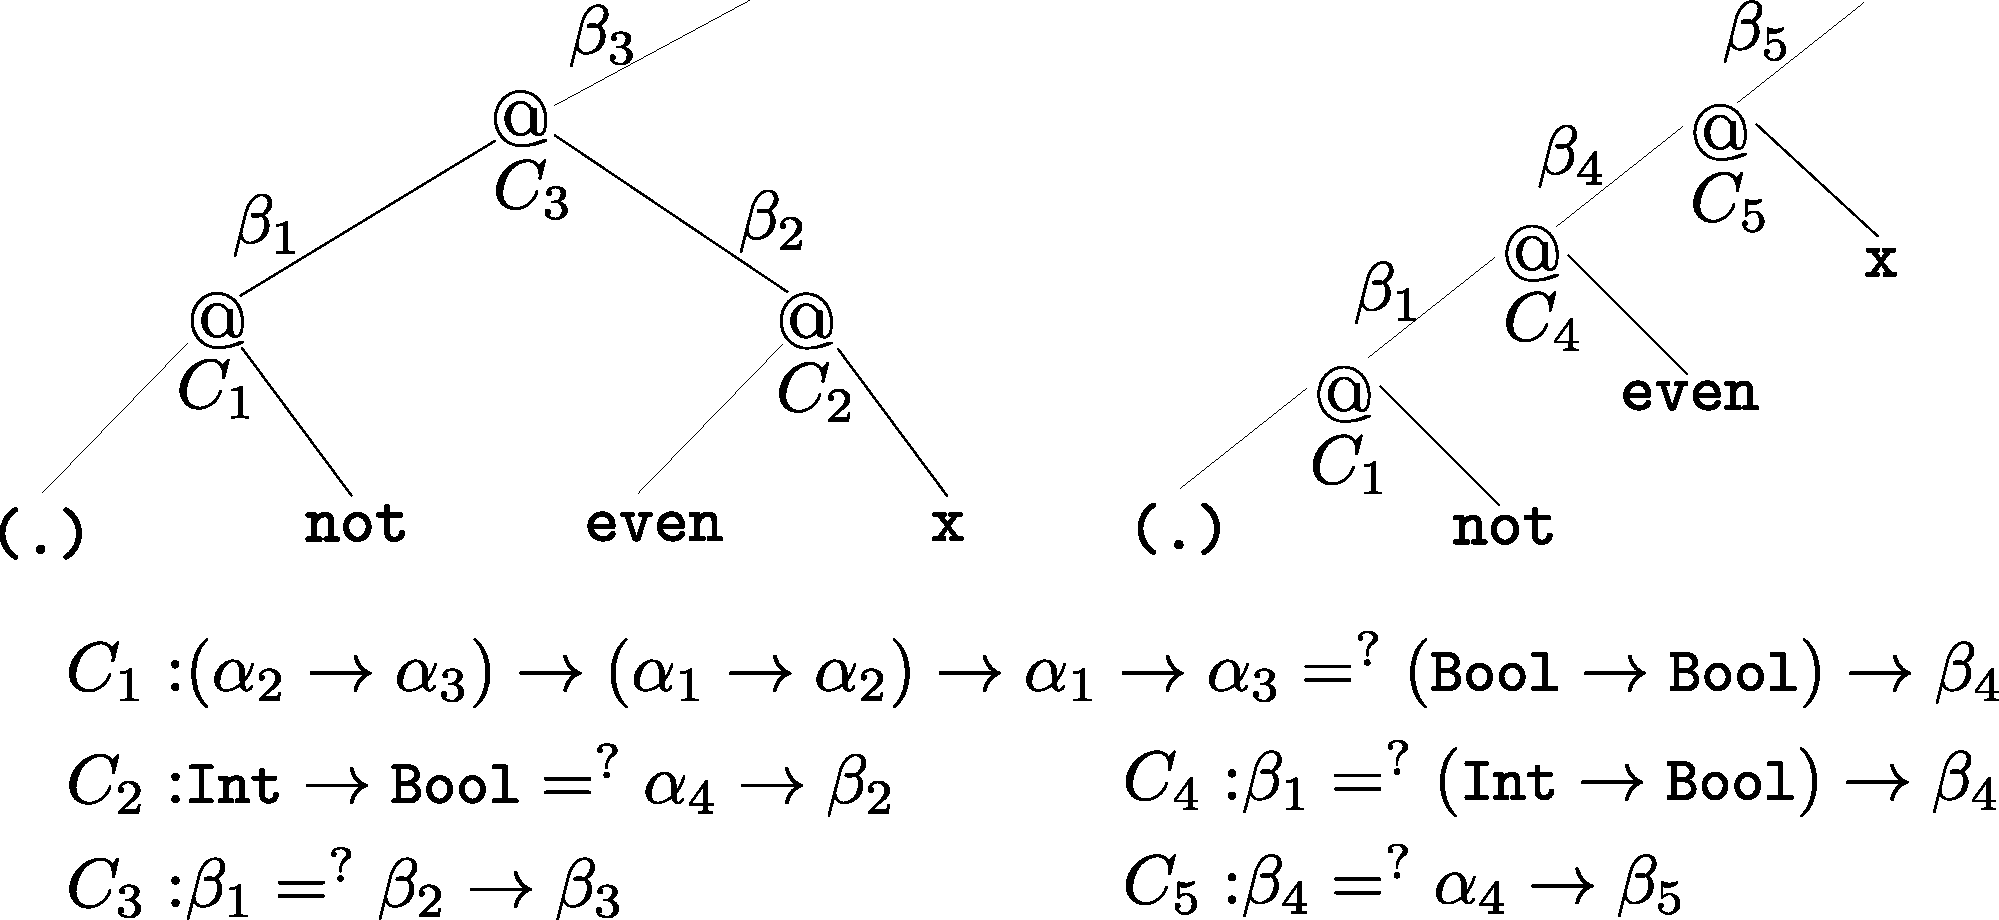
\includegraphics[width=0.85\columnwidth]{images/nonstruc.pdf}
\caption{The ASTs and constraints for \prog{not . even x} (left)
and \prog{(not . even) x} (right).
\ensuremath{@}s denote function applications.
The parameter \prog{x} has the type $\tvf$.
Annotations on edges denote types for the corresponding
subexpressions. For example, $\tvvf$ is the type for the
subexpression \prog{ (.) not}.}
\label{fig:nonstruc}
\end{figure}

A precondition for
constraint-based methods to work well is that the
faulty constraint is included in the given set of
constraints. However, this precondition fails
for the type errors caused by missing pairs of parentheses
or brackets.
For example,
consider debugging the type error for \prog{odd}
introduced in Section~\ref{sec:background:leaves:search}.
The \cs\ for \prog{odd} includes three constraints,
as shown in the left of Figure~\ref{fig:nonstruc}, where it
also presents the program AST. The constraints and AST for the
expected correct definition of \prog{odd} are shown in
the right of Figure~\ref{fig:nonstruc}. From the figure,
we observe that no constraint in \cs\ could be identified
as the faulty constraint such that changing the corresponding
subexpression would bring \prog{odd} to the
well-typed version, and consequently constraint-based debugging
methods fail to locate the real error cause. In this example,
both \toolH\ and \toolS\ blame the subexpression \prog{even x}
as the error cause.

%
For other non-leaf type causes, such as extra pairs
of parentheses, the precondition also fails to hold,
which makes constraint-based approach not work well.
We give evidence of this
for Helium in Section~\ref{xxx}.
%
In addition, constraint-based methods don't work well when there are
multiple error causes. One reason is that most
error debuggers try to report type errors in as few locations
as possible. As a result, even if the real error cause contains
multiple leaves, the debugger may return an error cause with
fewer leaves. For example, while the real error cause for
\prog{vulOp1} includes both \prog{(<)} and \prog{"~"},
Helium~\cite{Heeren05:TQT} suggests that the error cause
is \prog{replicate}.

Overall, constraint-based methods don't work well when a type
error is non-structural or involves multiple leaves.

\section{When Type Annotations Are Correct}
\label{sec:background:annotations}

While type inference can recover most omitted
type annotations, it is considered as a good
practice to add type annotations to at least
top-level bindings\footnote{http://en.wikibooks.org/wiki/Haskell/Type\_basics\#Type\_signatures\_in\_code}
for many reasons. As a form of documentation, type annotations improve
program readability. Compilers often exploit type annotations
to make type inference more efficient.

Type annotations also help to increase error
locating precision. For example,
the function \prog{vulOp} is
actually well typed if we remove its type annotation,
and it is the type annotation that helps error debuggers to detect
the type error in it. For this reason,
all GHC, Helium~\cite{Heeren03:HLH,Heeren05:TQT},
and \toolMin~\cite{Pavlinovic14:FMT,Pavlinovic15:PST}
treat user-specified type annotations as hard
constraints, meaning that they should always be trusted.
Once there is some error in type annotations, the
generated error messages is misleading, and following the
message will lead to more type errors in the program.
Thus, error debuggers work well when type annotations
are correct.

\chapter{Study Subjects}
\label{sec:subjects}

\section{Analyzed Datasets}
\label{sec:subjects:db}

\section{Finding the Reference Program}
\label{sec:subject:ref}

\section{Analysis Metrics}
\label{sec:subject:metric}


\chapter{Debugging Behavior Analysis}
\label{sec:analysis}

\section{Overview of Error Debugging in Practice}
\label{sec:overview}

\section{Where Were Error Causes?}
\label{sec:causes}

\section{Were Type Annotations Reliable?}
\label{sec:annotation}

\section{When Are Error Message Effective?}
\label{sec:effectiveness}

\section{What Language Features Are Difficult?}
\label{sec:difficulty}

\chapter{Nonstructural Type Error Representation}
\label{sec:features}

\section{Unifying Non-Unifiable Types}
\label{sec:features:unify}

\section{The Feature Vector}
\label{sec:features:feature}

\chapter{Learning Nonstructural Errors -- \newCompiler}
\label{sec:solution}

\section{Motivation for Using Machine Learning}
\label{sec:solution:motivation}

\section{The Proposed Approach}
\label{sec:solution:approach}

\subsection{Preliminaries of Machine Learning}

\subsection{Data Preprocessing}

\subsection{Imbalanced Classification}

\subsection{Implementation}

\section{Evaluation}
\label{sec:solution:eval}


\chapter{Conclusion and Future Work}
\label{sec:conclusion}

\section{Other Applications}
\label{sec:conclusion:other}

\section{Main Contributions and Future Directions}
\label{sec:conclusion:close}

%\include{chapter11}	

%\include{chapter12}	
%
% Appendix/Appendices
%
% If you have only one appendix, use the command \appendix instead
% of \appendices.
%
%\appendices

%\include{chapter-appendix1}
%\include{chapter-appendix2}
%\include{chapter-appendix3}

%
% Generate the bibliography.
%

%\nocite{*}      % This command causes all items in the               %
                % bibliographic database to be added to              %
                % the bibliography, even if they are not             %
                % explicitly cited in the text.                      %

% Here the bibliography is inserted.
% Replace "example" with the name of your ".bib" file
\bibliography{error-reporting,me,paper,pldi}                      
\index{Bibliography@\emph{Bibliography}}
%


%
% Generate the index.
% 
%
\printindex     % Include the index here. Comment out this line      
%               % with a percent sign if you do not want an index .  
%

\begin{abstract}
test
\end{abstract}

\end{document}
% The following comment block is used by the different flavors of EMACS and
% the AUCTEX package to manage multiple documents.  In order for AUCTEX
% to understand you're working with multiple files, you should define
% the TeX-master variable as a file local variable that identifies your
% master document.
%
% Please do not remove.
%%% Local Variables: 
%%% mode: latex
%%% TeX-master: "example.tex"
%%% End: 
